\paragraph{Цель работы:} формирование заданной формы используя CNC симулятор G-кода.

\subsection*{Задание}

Построить форму, заданную на рисунке \ref{fig:task}.

\begin{figure}[ht]
    \centering
    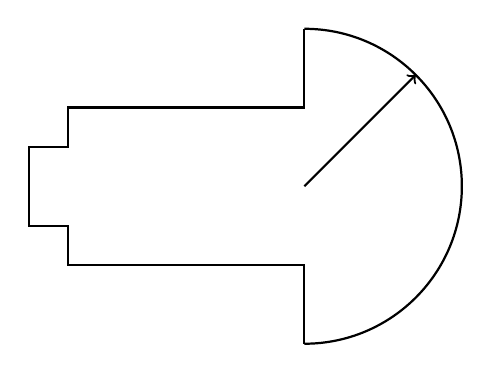
\begin{tikzpicture}[thick]
        %Coordinates
        \coordinate (A) at (3.5,2);
        \coordinate (B) at (3.5,1);
        \coordinate (C) at (0.5,1);
        \coordinate (D) at (0.5,0.5);
        \coordinate (E) at (0,0.5);
        \coordinate (F) at (0,0);
        \coordinate (R1) at (3.5,0);
        \coordinate (R2) at (4.9142,1.4142);
        %Arcs
        \draw (A) arc (90:-90:2cm);
        %Lines
        \draw (A)--(B)--(C)--(D)--(E)--(F);
        \draw ([yscale=-1]A)--([yscale=-1]B)--([yscale=-1]C)--([yscale=-1]D)--([yscale=-1]E)--(F);
        %Dimensions
        \draw[->] (R1)--(R2);
        \tkzLabelSegment[above=0.7ex](B,C){30}
        \tkzLabelSegment[below right](R1,R2){20}
        \tkzLabelSegment[left](E,[yscale=-1]E){10}
    \end{tikzpicture}
    \caption{Задание\label{fig:task}}
\end{figure}

\subsection*{Исходный код}

Исходный код формирования детали заданной формы:

\begin{verbatim}
    N0010 G54 G92 X0.000 Z70.000
    N0020 G59
    N0030 G00 X60.000 Z60.000
    N0040 T0303
    N0050 G00 X30.000 Z0.000
    N0060 G01 X0.000 Z0.000
    N0070 G03 X20.000 Z-20.000 K-20.000
    N0080 T0707
    N0090 G01 X10
    N0100 G01 Z-50
    N0110 G01 X5
    N0120 G01 Z-55
    N0130 G01 X0
    N0160 G01 X30
    N0170 G00 X60.000 Z60.000
    N0180 G53 G56 T0000 M30
\end{verbatim}

Результат выполнения программы можно наблюдать на рисунке \ref{fig:done}.

\begin{figure}[ht]
\centering
	\includegraphics[height=.7\linewidth,angle=90]{1.png}
    \caption{Построение заданной дуги\label{fig:done}}
\end{figure}

\subsection*{Выводы}

В лабораторной работе мы применили знания различных команд на практике, сформировав деталь определенной формы. В процессе обработки мы сменили инструмент на седьмой для возможности обработки без врезания нережущей части инструмента в необрабатываемую часть детали.

\clearpage
